\begin{song}{title=\predtitle\centering Kutil \\\large Chinaski  \vspace*{-0.3cm}}  %% sem se napíše jméno songu a autor
\begin{centerjustified}
\nejvetsi

\sloka
Jsem ^{E}kutil.

Mám malou ^{F#mi}dílnu, víc mě ^{A{\color{white}\_\_}E}nezajímá,

mé ^{E{\color{white}\_}}hobby je moje práce,

šťastnej ^{F#mi}člověk každej, ^{A}kdo to ^{{\color{white}\_}E}tak má.

Mám ^{E}ženu.

Je mladá, ^{F#mi}krásná, chytrá, ^{A{\color{white}\_\_}E}přívětivá.

Má jednu malinkatou ^{E{\color{white}\_}}chybu,

že si ^{F#mi\z}se~mnou vůbec ^{A{\color{white}\_\_}E}nepovídá.

\refren
A tak ^{F#mi}hledám holku sdílnou,

co by chtěla kluka s dílnou,

^{A}abych nebyl ^{H}sám. ^{H7}

\textbf{E  F\sharp mi  A  E  C\sharp mi  A  G  D  E }

\sloka
Jsem kutil.

Mám malou dílnu, víc mě nezajímá.

Má práce je moje hobby,

šťastnej člověk každej, kdo to tak má.

Mám ženu.

Je mladá, krásná, chytrá, přívětivá.

Má jednu malinkatou chybu,

že si se mnou vůbec nepovídá.

\refren

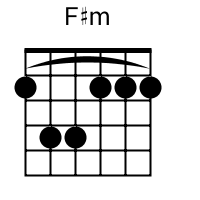
\includegraphics[width=3cm]{../Akordy/fxm.png}
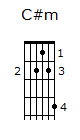
\includegraphics[width=3cm]{../Akordy/cxm.png}

\end{centerjustified}
\setcounter{Slokočet}{0}
\end{song}
